\documentclass[12pt]{article}

\usepackage{fontawesome}
\usepackage{hyperref}
\usepackage{xurl}
\usepackage{graphicx}
\usepackage{float}
\usepackage[tagged, highstructure]{accessibility}
\usepackage{bookmark}
\usepackage{enumitem}

\hypersetup{
    colorlinks=false,
    pdfborder={0 0 0},
    pdftitle={Data Visualization},
    pdfauthor={Adrianna Holden-Gouveia},
    pdfsubject={Advanced Data - Lab Assignment},
    pdflang={en-US},
    pdfkeywords={data visualization, charts, graphs, AI visualization, data presentation}
}

% Configure PDF bookmarks for navigation
\bookmarksetup{
    numbered,
    open,
}

% Configure list spacing for better accessibility
\setlist{nosep}



\title{Data Visualization}
\author{
        Adrianna Holden-Gouveia \\
        Website: \href{https://aholdengouveia.name}{aholdengouveia.name}\\ 
        \date{\vspace{-5ex}}
        %Email: \href{mailto:admin@aholdengouveia.name}{admin@aholdengouveia.name} \\
%        \faLinkedin{: aholdengouveia} \\
        \faGithub {: aholdengouveia} \\
        %\faTwitter {: aholdengouveia} \\
        }

%S\date{\today}


\begin{document}    

\maketitle

%\begin{abstract}
%This is a template for Linux Administration Lab work
%\end{abstract}
%\tableofcontents


\section*{Accessibility Notice}
This document is also available in HTML format at:

Link: \href{https://aholdengouveia.name/AdvData/labs/wk13dataviz.html}{\textbf{\nolinkurl{https://aholdengouveia.name/AdvData/labs/wk13dataviz.html}}}

The HTML version provides enhanced accessibility features including keyboard navigation, screen reader support, responsive design, dark mode support, and high contrast options.

\section*{Request}
\noindent\textbf{Request:} DATA-6874\\
\textbf{Requested by:} Operations manager at your company\\
\textbf{Data:} Your database, and your documented queries from the SQL Review labs

\section*{Background}
Your manager has read your documented queries, but tables of numbers are hard to take into a meeting. They want charts that answer two of your business questions clearly and honestly, and that everyone on the team can read, including people who use screen readers or can't tell some colours apart.

\section*{Learning Outcomes}
By the end of this lab, you will be able to:
\begin{itemize}
    \item Create data visualizations from database query results
    \item Evaluate visualizations using a checklist, and choose the best one for an audience
    \item Identify how a visualization can mislead, and how to avoid it
    \item Make visualizations accessible, with alt text and without relying on colour alone
\end{itemize}

\section*{Lab Instructions}
Use your own data set and database. Books are my example data only.

To make charts, you need your query results in a spreadsheet. You can use any spreadsheet tool, such as Google Sheets, which you used in Introduction to Data, or Excel. Two ways to get your results into a spreadsheet, both linked under Resources:
\begin{itemize}
    \item Suggested: use the Turn query results into a CSV file section of my CSV to Database Converter. Choose your database file, run your query, and download the results as a CSV file. Then open it in your spreadsheet tool.
    \item Also suggested, for small results: run your query in SandboxSQL, then select the results, copy them, and paste them into your spreadsheet.
\end{itemize}

\subsection*{Screenshots}
Several parts of this lab ask for a screenshot. Each screenshot should have your name, term, and year.  One of the easiest ways to do that is make a text document with your name and term/year on your computer and save it to use all term. Any screenshots that don't include this information won't be counted.

\begin{figure}[H]
    \centerline{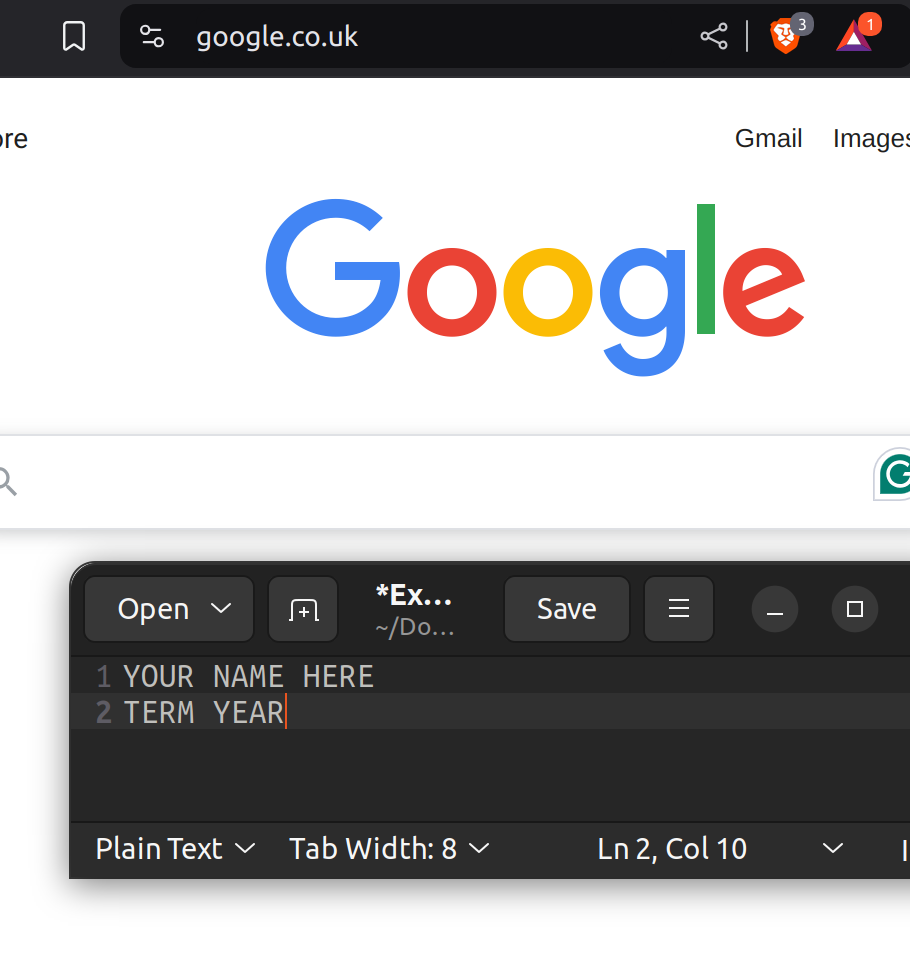
\includegraphics[scale=.2]{ExampleScreenshot.png}}
    \caption{This is an image of what each of your screenshots should look like}
    \alt{Example screenshot: a web browser showing the Google home page, with a small text editor window in front of it that says YOUR NAME HERE and TERM YEAR}
\end{figure}

\subsection*{Part 1: Get Your Data}
\begin{enumerate}
    \item Pick 2 of your business questions from the SQL Review labs whose answers would make a good chart. Queries that count, total, or average things by group usually work best. You can update a query, or write a new one, to answer the question better. GROUP BY, which you used in the SQL Scaling lab, is often useful here.
    \item Take a screenshot of each query and its results.
\end{enumerate}

\subsection*{Part 2: Automatic and Designed Charts}
For each of your 2 questions, make 2 charts, for 4 charts in total:
\begin{enumerate}
    \item An automatic chart: select your data, insert a chart, and keep whatever chart the tool picks, without changing anything.
    \item A designed chart: choose the chart type, title, axis labels, colours, and any notes on purpose, to answer the business question as clearly as you can.
\end{enumerate}
For each designed chart, explain why you chose that chart type, and what you changed from the automatic chart and why.

\subsection*{Part 3: Evaluate Your Charts}
\begin{enumerate}
    \item Evaluate all 4 charts with the data visualization checklist (linked under Resources), on all 7 points. If a point doesn't apply, explain why not.
    \item For each question, which of the 2 charts would you show your manager, and why?
    \item Check the numbers in each chart against your query results. Does each chart show your data accurately?
\end{enumerate}

\subsection*{Part 4: A Misleading Chart}
Make a misleading version of one of your designed charts, on purpose. For example, start the axis above zero so small differences look huge, show an average that hides a big spread, leave out some of the data, or use 3D so sizes are hard to compare.
\begin{enumerate}
    \item Show your original chart and the misleading version side by side.
    \item Explain what makes it misleading, and how someone could be fooled by it.
    \item What business decision could go wrong if your manager believed the misleading chart?
\end{enumerate}

\subsection*{Part 5: Accessibility}
For the 2 charts you'd show your manager:
\begin{enumerate}
    \item Write alt text: 1 or 2 sentences that give the main point of the chart, not just what kind of chart it is. For example, ``Bar chart of books by genre. Classics is by far the biggest group, with 50 of 99 books, about three times as many as Fiction, the next biggest.''
    \item Check that your chart doesn't rely on colour alone. If it were printed in black and white, could you still tell everything apart? If not, add data labels or direct labels, and show the updated chart.
    \item Check the contrast of any coloured text against its background with the WebAIM Contrast Checker (linked under Resources), and give the result.
\end{enumerate}

\section*{Acceptance Criteria}
This request is done when:
\begin{itemize}
    \item 2 business questions, each with a query and a screenshot of its results
    \item 4 charts: an automatic and a designed chart for each question, with your reasons for each designed chart
    \item All 4 charts are evaluated on all 7 checklist points
    \item You've chosen a chart for each question and checked its numbers against your query results
    \item Your misleading chart is shown beside the original, with what misleads, how, and the business risk
    \item Your 2 chosen charts have alt text that gives the main point, a colour check, and a contrast check
    \item Every screenshot follows the screenshot rules
\end{itemize}

\section*{Deliverables}
One file that includes Parts 1 to 5.

Audience: your manager, the operations manager.

\section*{Resources}
References, a video, a PowerPoint and some notes are available at my website
Link: \href{https://www.aholdengouveia.name/AdvData/Datavis.html}{\textbf{\nolinkurl{https://www.aholdengouveia.name/AdvData/Datavis.html}}}

Data visualization checklist
Link: \href{https://www.aholdengouveia.name/AdvData/labs/DataVizChecklist.docx}{\textbf{\nolinkurl{https://www.aholdengouveia.name/AdvData/labs/DataVizChecklist.docx}}}

My CSV to Database Converter, for turning query results into a CSV file
Link: \href{https://www.aholdengouveia.name/AdvData/labs/csv-to-database.html}{\textbf{\nolinkurl{https://www.aholdengouveia.name/AdvData/labs/csv-to-database.html}}}

SandboxSQL, for running your queries
Link: \href{https://www.sandboxsql.com/}{\textbf{\nolinkurl{https://www.sandboxsql.com/}}}

Help for making charts in Google Sheets
Link: \href{https://support.google.com/docs/answer/63824}{\textbf{\nolinkurl{https://support.google.com/docs/answer/63824}}}

Help for making charts in Excel
Link: \href{https://support.microsoft.com/en-us/office/create-a-chart-from-start-to-finish-0baf399e-dd61-4e18-8a73-b3fd5d5680c2}{\textbf{\nolinkurl{https://support.microsoft.com/en-us/office/create-a-chart-from-start-to-finish-0baf399e-dd61-4e18-8a73-b3fd5d5680c2}}}

WebAIM Contrast Checker
Link: \href{https://webaim.org/resources/contrastchecker/}{\textbf{\nolinkurl{https://webaim.org/resources/contrastchecker/}}}

\end{document}